%!TEX root = pixelrnn.tex
\section{Pixel Recurrent Neural Networks}
\label{sect:pixelrnn}

In this section we describe the architectural components that compose the {PixelRNN}. In Sections \ref{sect:row_lstm} and \ref{sect:diag_lstm}, we describe the two types of LSTM layers that use convolutions to compute at once the states along one of the spatial dimensions. 
In Section \ref{sect:residual} we describe how to incorporate \emph{residual} connections to improve the training of a PixelRNN with many LSTM layers.  In Section \ref{sect:masked} we describe the softmax layer that computes the {discrete} joint distribution of the colors and the masking technique that ensures the proper conditioning scheme. In Section \ref{sect:pixelcnn} we describe the PixelCNN architecture. Finally in Section \ref{sect:multiscale} we describe the multi-scale architecture.

\begin{figure}
\centering
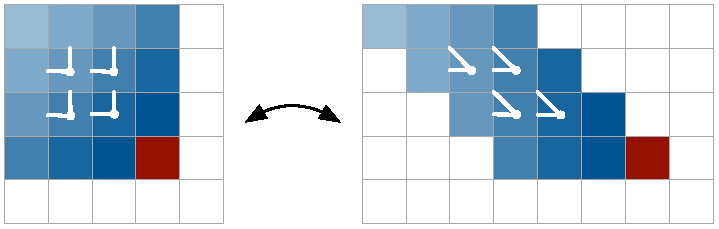
\includegraphics[width=0.46\textwidth]{bilstm.pdf}
\vspace{-0.3cm}
\caption{In the Diagonal BiLSTM, to allow for parallelization along the diagonals, the input map is skewed by offseting each row by one position with respect to the previous row. When the spatial layer is computed left to right and column by column, the output map is shifted back into the original size. The convolution uses a kernel of size $2 \times 1$. }
\label{fig:bilstm}
\vspace{-0.3cm}
\end{figure}

\subsection{Row LSTM}
\label{sect:row_lstm}

The Row LSTM is a unidirectional layer that processes the image row by row from top to bottom computing features for a whole row at once; the computation is performed with a one-dimensional convolution. For a pixel $x_i$ the layer captures a roughly triangular context above the pixel as shown in Figure \ref{mappings} (center). The kernel of the one-dimensional convolution has size $k \times 1$ where $k \geq 3$; the larger the value of $k$ the broader the context that is captured. The weight sharing in the convolution ensures translation invariance of the computed features along each row.

The computation proceeds as follows. An LSTM layer has an {input-to-state} component and a recurrent {state-to-state} component that together determine the four gates inside the LSTM core. To enhance parallelization in the Row LSTM the input-to-state component is first computed for the entire two-dimensional input map; for this a $k \times 1$ convolution is used to follow the row-wise orientation of the LSTM itself. The convolution is \emph{masked} to include only the valid context (see Section \ref{sect:masked}) and produces a tensor of size $4h \times n \times n$, representing the four gate vectors for each position in the input map, where $h$ is the number of output feature maps.

 To compute one step of the state-to-state component of the LSTM layer, one is given the previous hidden and cell states $\vec{h}_{i-1}$ and $\vec{c}_{i-1}$, each of size $h \times n \times 1$. The new hidden and cell states $\vec{h}_i$, $\vec{c}_i$ are obtained as follows:

 \vspace{-0.2cm}
 \begin{equation}
 \begin{split}
 [\vec{o}_i, \vec{f}_i, \vec{i}_i, \vec{g}_i ] & = \sigma (\vec{K}^{ss} \circledast \vec{h}_{i-1} + \vec{K}^{is} \circledast \vec{x}_{i}) \\
\vec{c}_i & = \vec{f}_i \odot \vec{c}_{i-1} + \vec{i}_i \odot \vec{g}_i \\
\vec{h}_i & = \vec{o}_i \odot \tanh(\vec{c}_i)\\
\end{split}
\label{eq:lstm}
 \vspace{-0.3cm}
 \end{equation}

where $\vec{x}_i$ of size $h \times n \times 1$ is row $i$ of the input map, and $\circledast$ represents the convolution operation and $\odot$ the element-wise multiplication. The weights $\vec{K}^{ss}$ and $\vec{K}^{is}$ are the kernel weights for the state-to-state and the input-to-state components, where the latter is precomputed as described above. In the case of the output, forget and input gates $\vec{o}_i$, $\vec{f}_i$ and $\vec{i}_i$, the activation $\sigma$ is the logistic sigmoid function, whereas for the content gate $\vec{g}_i$, $\sigma$ is the $\tanh$ function. Each step computes at once the new state for an entire row of the input map. Because the Row LSTM has a triangular receptive field (Figure \ref{mappings}), it is unable to capture the entire available context.

\begin{figure}[ht]
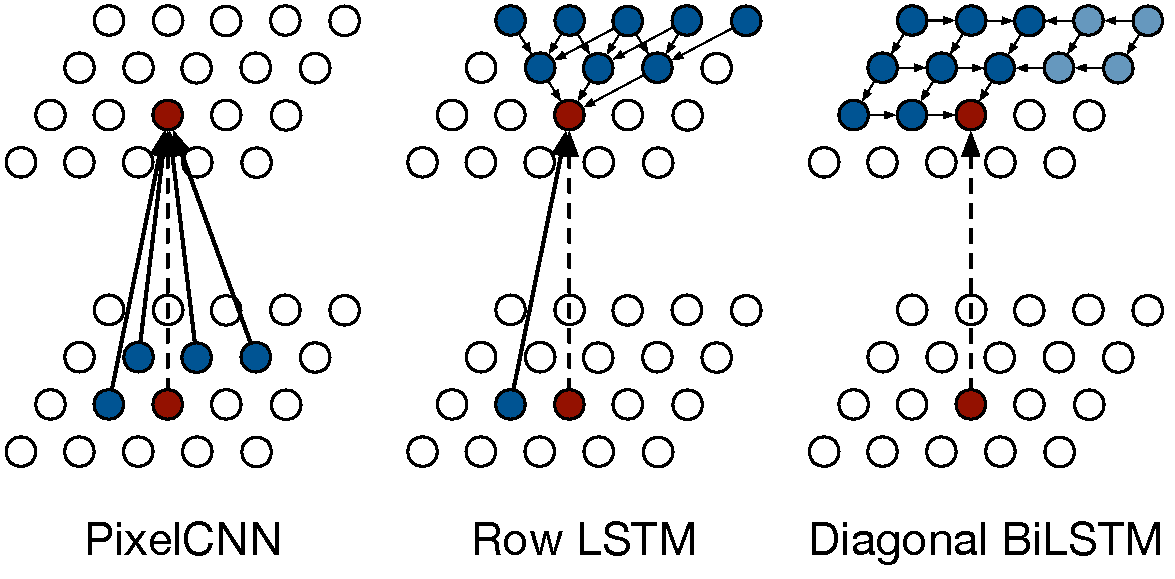
\includegraphics[width=0.48\textwidth]{graphs3.pdf}
\vspace{-0.7cm}
\caption{Visualization of the input-to-state and state-to-state mappings for the three proposed architectures.}
\label{mappings}
\vspace{-0.2cm}
\end{figure}

\subsection{Diagonal BiLSTM}
\label{sect:diag_lstm}

The Diagonal BiLSTM is designed to both parallelize the computation and to capture the entire available context for any image size. Each of the two directions of the layer scans the image in a diagonal fashion starting from a corner at the top and reaching the opposite corner at the bottom. Each step in the computation computes at once the LSTM state along a diagonal in the image. Figure \ref{mappings} (right) illustrates the computation and the resulting receptive field.

The diagonal computation proceeds as follows. We first skew the input map into a space that makes it easy to apply convolutions along diagonals. The {skewing} operation offsets each row of the input map by one position with respect to the previous row, as illustrated in Figure \ref{fig:bilstm}; this results in a map of size $n \times (2n-1)$. At this point we can compute the input-to-state and state-to-state components of the Diagonal BiLSTM. For each of the two directions, the input-to-state component is simply a $1 \times 1$ convolution $K^{is}$ that contributes to the four gates in the LSTM core; the operation generates a $4 h \times n \times n$ tensor. The state-to-state recurrent component is then computed with a \emph{column-wise} convolution $K^{ss}$ that has a kernel of size $2 \times 1$. The step takes the previous hidden and cell states, combines the contribution of the input-to-state component and produces the next hidden and cell states, as defined in Equation \ref{eq:lstm}. The output feature map is then skewed back into an $n \times n$ map by removing the offset positions. This computation is repeated for each of the two directions. Given the two output maps, to prevent the layer from seeing future pixels, the \emph{right} output map is then shifted down by one row and added to the \emph{left} output map.
 
Besides reaching the full dependency field, the Diagonal BiLSTM has the additional advantage that it uses a convolutional kernel of size $2\times1$ that processes a minimal amount of information at each step yielding a highly non-linear computation. Kernel sizes larger than $2\times1$ are not particularly useful as they do not broaden the already global receptive field of the Diagonal BiLSTM. 

\subsection{Residual Connections}
\label{sect:residual}

We train PixelRNNs of up to twelve layers of depth. As a means to both increase convergence speed and propagate signals more directly through the network, we deploy \emph{residual connections} \cite{DBLP:journals/corr/HeZRS15} from one LSTM layer to the next. Figure \ref{fig:residual_blocks} shows a diagram of the residual blocks. The input map to the PixelRNN LSTM layer has $2h$ features. The input-to-state component reduces the number of features by producing $h$ features per gate. After applying the recurrent layer, the output map is upsampled back to $2h$ features per position via a $1\times1 $ convolution and the input map is added to the output map. This method is related to previous approaches that use gating along the depth of the recurrent network \cite{DBLP:journals/corr/KalchbrennerDG15,zhang2016highway}, but has the advantage of not requiring additional gates. Apart from residual connections, one can also use learnable skip connections from each layer to the output. In the experiments we evaluate the relative effectiveness of residual and layer-to-output skip connections. 
	
\begin{figure}[ht]
\centering
\begin{subfigure}{.4\textwidth}
  \centering
  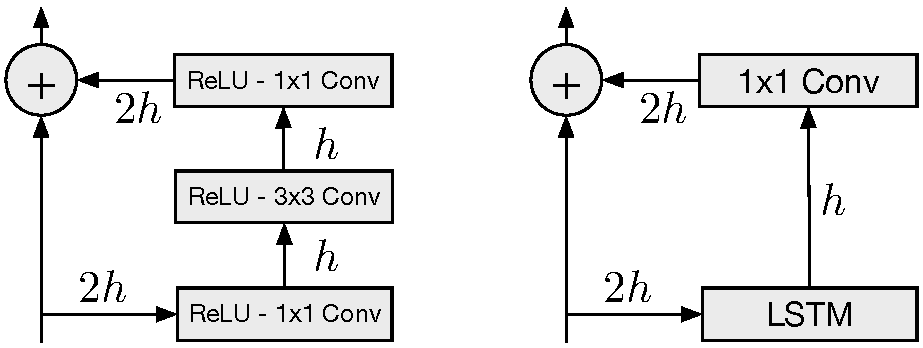
\includegraphics[width=\linewidth]{residuals2.pdf}
\end{subfigure}%
\caption{Residual blocks for a PixelCNN (left) and PixelRNNs.}
\label{fig:residual_blocks}
\vspace{-0.2cm}
\end{figure}

\subsection{Masked Convolution}
\label{sect:masked}

The $h$ features for each input position at every layer in the network are split into three parts, each corresponding to one of the RGB channels. When predicting the R channel for the current pixel $x_i$, only the generated pixels left and above of $x_i$ can be used as context. When predicting the G channel, the value of the R channel can also be used as context in addition to the previously generated pixels. Likewise, for the B channel, the values of both the R and G channels can be used. To restrict connections in the network to these dependencies, we apply a \emph{mask} to the input-to-state convolutions and to other purely convolutional layers in a PixelRNN. 

We use two types of masks that we indicate with \emph{mask A} and \emph{mask B}, as shown in Figure \ref{depen} (Right). Mask A is applied only to the first convolutional layer in a PixelRNN and restricts the connections to those neighboring pixels and to those colors in the current pixels that have already been predicted. On the other hand, mask B is applied to all the subsequent input-to-state convolutional transitions and relaxes the restrictions of mask A by also allowing the connection from a color to itself. The masks can be easily implemented by zeroing out the corresponding weights in the input-to-state convolutions after each update. Similar masks have also been used in variational autoencoders \cite{gregor2013deep, germain2015made}.

\begin{table}[t]
\small
	\begin{center}
	\begin{tabular}{l|l|l}
		\toprule
		\multicolumn{1}{c|}{\textbf{ PixelCNN} }& \multicolumn{1}{c|}{\textbf{ Row LSTM} } & \multicolumn{1}{|c}{\textbf{ Diagonal BiLSTM} }  \\ \midrule
		\multicolumn{3}{c}{ $7 \times 7$ conv mask A} \\ \midrule 
		\multicolumn{3}{c}{ \textbf{Multiple residual blocks:} (see fig \ref{fig:residual_blocks})} \\ 
		\multicolumn{3}{c}{ } \\ 
	    \multirow{3}{*}{}Conv & Row LSTM & Diagonal BiLSTM \\ % & 
	    				 $3 \times 3$  mask B & i-s: $3 \times 1$ mask B & i-s: $1\times1$ mask B \\
	    				 & s-s: $3 \times 1$ no mask & s-s: $1\times2$ no mask \\ \midrule
	    \multicolumn{3}{c}{ ReLU followed by $1 \times 1$ conv, mask B (2 layers)} \\ \midrule
	    \multicolumn{3}{c}{ 256-way Softmax for each RGB color (Natural images)}\\
	    \multicolumn{3}{c}{ or Sigmoid (MNIST)} \\ 
	    \bottomrule
	\end{tabular}
	\end{center}
\vspace{-0.2cm}
\caption{Details of the architectures. In the LSTM architectures i-s and s-s stand for input-state and state-state convolutions.}
\vspace{-0.3cm}
\label{table:architectures}
\end{table}

\subsection{PixelCNN}
\label{sect:pixelcnn}

The Row and Diagonal LSTM layers have a potentially unbounded dependency range within their receptive field. This comes with a computational cost as each state needs to be computed sequentially. One simple workaround is to make the receptive field large, but not unbounded. We can use standard convolutional layers to capture a bounded receptive field and compute features for all pixel positions at once. The PixelCNN uses multiple convolutional layers that preserve the spatial resolution; pooling layers are not used. Masks are adopted in the convolutions to avoid seeing the future context; masks have previously also been used in non-convolutional models such as MADE \cite{germain2015made}. Note that the advantage of parallelization of the PixelCNN over the PixelRNN is only available during training or during evaluating of test images. The image generation process is sequential for both kinds of networks, as each sampled pixel needs to be given as input back into the network.

\subsection{Multi-Scale PixelRNN}
\label{sect:multiscale}

The Multi-Scale PixelRNN is composed of an \emph{unconditional} PixelRNN and one or more \emph{conditional} PixelRNNs. The unconditional network first generates in the standard way a smaller $s \times s$ image that is \emph{subsampled} from the original image. The conditional network then takes the $s \times s$ image as an additional input and generates a larger $n\times n$ image, as shown in Figure \ref{depen} (Middle).

The conditional network is similar to a standard PixelRNN, but each of its layers is biased with an upsampled version of the small $s \times s$ image. The upsampling and biasing processes are defined as follows. In the upsampling process, one uses a convolutional network with deconvolutional layers to construct an enlarged feature map of size $c \times n \times n$, where $c$ is the number of features in the output map of the upsampling network. Then, in the biasing process, for each layer in the conditional PixelRNN, one simply maps the $c \times n \times n$ conditioning map into a $4h \times n \times n$ map that is added to the input-to-state map of the corresponding layer; this is performed using a $1 \times 1$ unmasked convolution. The larger $n \times n$ image is then generated as usual.


\section{Specifications of Models}

In this section we give the specifications of the PixelRNNs used in the experiments. We have four types of networks: the PixelRNN based on Row LSTM, the one based on Diagonal BiLSTM, the fully convolutional one and the Multi-Scale one. 

Table \ref{table:architectures} specifies each layer in the single-scale networks. The first layer is a $7\times7$ convolution that uses the mask of type A. The two types of LSTM networks then use a variable number of recurrent layers. The input-to-state convolution in this layer uses a mask of type B, whereas the state-to-state convolution is not masked. The PixelCNN uses convolutions of size $3\times3$ with a mask of type B. The top feature map is then passed through a couple of layers consisting of a Rectified Linear Unit (ReLU) and a $1\times1$ convolution. For the CIFAR-10 and ImageNet experiments, these layers have 1024 feature maps; for the MNIST experiment, the layers have 32 feature maps. Residual and layer-to-output connections are used across the layers of all three networks.

The networks used in the experiments have the following hyperparameters. For MNIST we use a Diagonal BiLSTM with 7 layers and a value of $h=16$  (Section \ref{sect:residual} and Figure \ref{fig:residual_blocks} right). For CIFAR-10 the Row and Diagonal BiLSTMs have 12 layers and a number of $h=128$ units. The PixelCNN has 15 layers and $h=128$. For $32\times32$ ImageNet  we adopt a 12 layer Row LSTM with $h=384$ units and for $64\times64$ ImageNet we use a 4 layer Row LSTM with $h=512$ units; the latter model does not use residual connections. 
